\section{Einfache Bestimmung der Brennweite einer Linse}

\begin{figure}[ht]
    \centering
    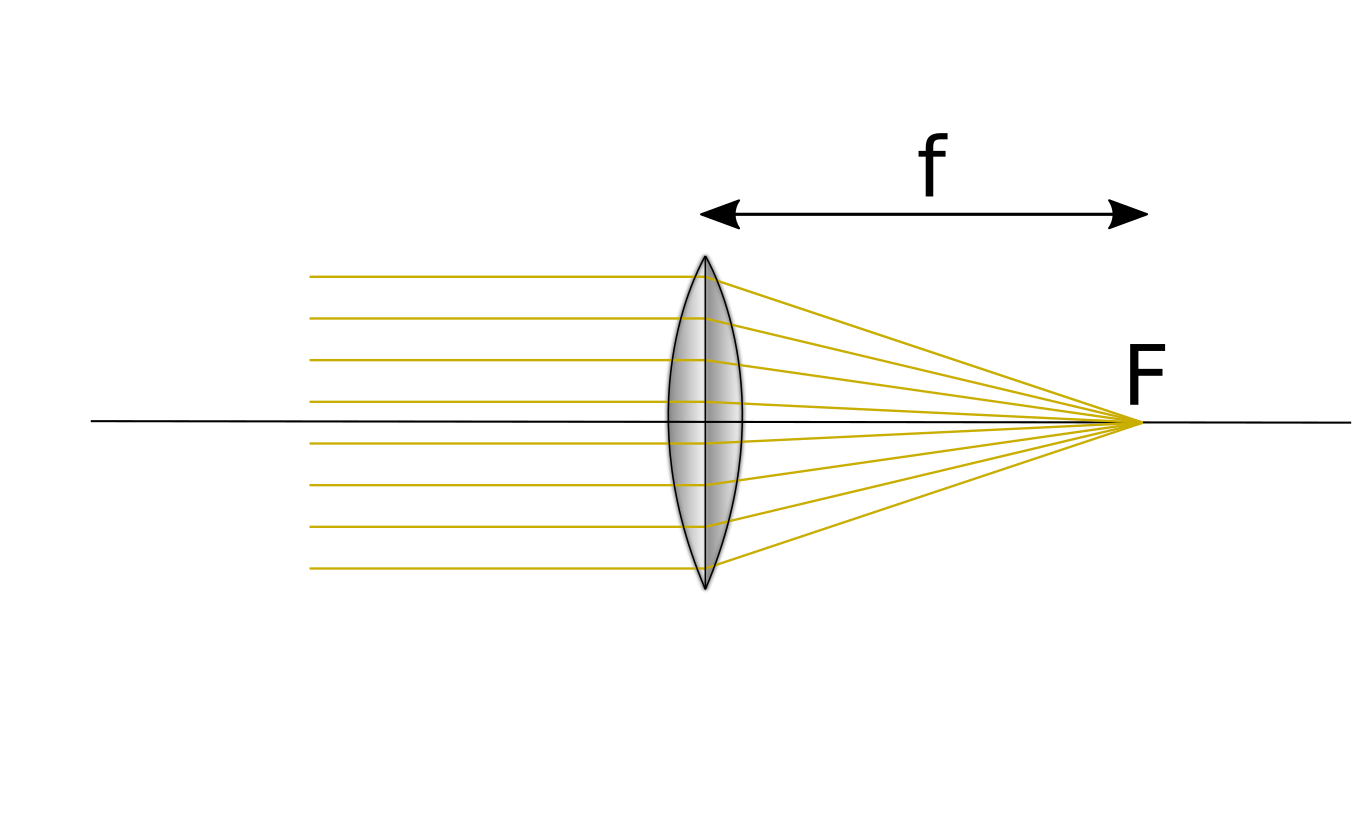
\includegraphics[scale=0.8]{Geometrische_Optik/Protokoll/fig/Versuch1.1.png}
    \caption{Einfach Bestimmung der Brennweite einer Linse}
    \label{fig:Versuch1.1}
\end{figure}

In diesem Versuchsteil soll die Brennweite einer Linse nur mit Hilfe eines Maßstabs und eines Schirms kontrolliert werden. Dazu werden sowohl Linse als auch Schirm auf einer optischen Bank montiert (Abb. \ref{fig:Versuch1.1}). Um den Fehler bei dieser Messung zu minimieren wird der Abstand zwischen Lichtquelle groß gewählt bzw. gegebenenfalls ein Kondensor nach der Lichtquelle zwischengeschaltet. Für die Messung wird nun die Linse solange verschoben, bis ein möglichst kleiner Lichtpunkt auf dem Schirm entsteht. Der Abstand zwischen Schirm und der Linse ist somit die Brennweite. Für den Versuch wird eine Linse mit einer angegebenen Brennweite von $F = 15 cm$ gewählt, dabei wird der Schirm auf der 195cm-Marke der optischen Bank fixiert. Es ergeben sich die Werte in der Tabelle \ref{tab:Daten1}. Somit ergibt sich ein Mittelwert von $16.5600$ mit einer Standardabweichung von $0.066cm$, also: $16.5600cm \pm 0.066cm$. Dies entspricht einer Abweichung von ca. $9 \% $ zum angegebenen Wert. Diese Abweichung liegt in der Ungenauigkeit der Messmethode begründet. Faktoren, die die Genauigkeit der Messung beeinflussen sind etwa, dass die Messung nicht mit monochromatischem Licht durchgeführt wurde, denn die Brechzahl hängt von der Wellenlänge des Lichts ab. Allerdings wurden zehn dicht aneinander liegende Werte ermittelt, was auch auf eine nicht korrekte Angabe der Brennweite auf der Linse hindeuten könnte.
 
\begin{table}[h!]
    \centering
    \begin{tabular}{|c|c|}
    	\hline
    	Messung Nr. & Pos. Linse (cm) \\
    	\hline
    	1 & 178.5 \\
    	\hline
    	2 & 178.4 \\
    	\hline
    	3 & 178.4 \\
    	\hline
    	4 & 178.4 \\
    	\hline
    	5 & 178.5 \\
    	\hline
    	6 & 178.4 \\
    	\hline
    	7 & 178.5 \\
    	\hline
    	8 & 178.3 \\
    	\hline
    	9 & 178.5 \\
    	\hline
    	10 & 178.5 \\
    	\hline
    
    \end{tabular}
    \caption{Daten: Einfache Bestimmung der Brennweite einer Linse}
    \label{tab:Daten1}
\end{table}

\section{Brennweitenbestimmung einer Linse mit dem Besselverfahren}

\begin{figure}[h]
    \centering
    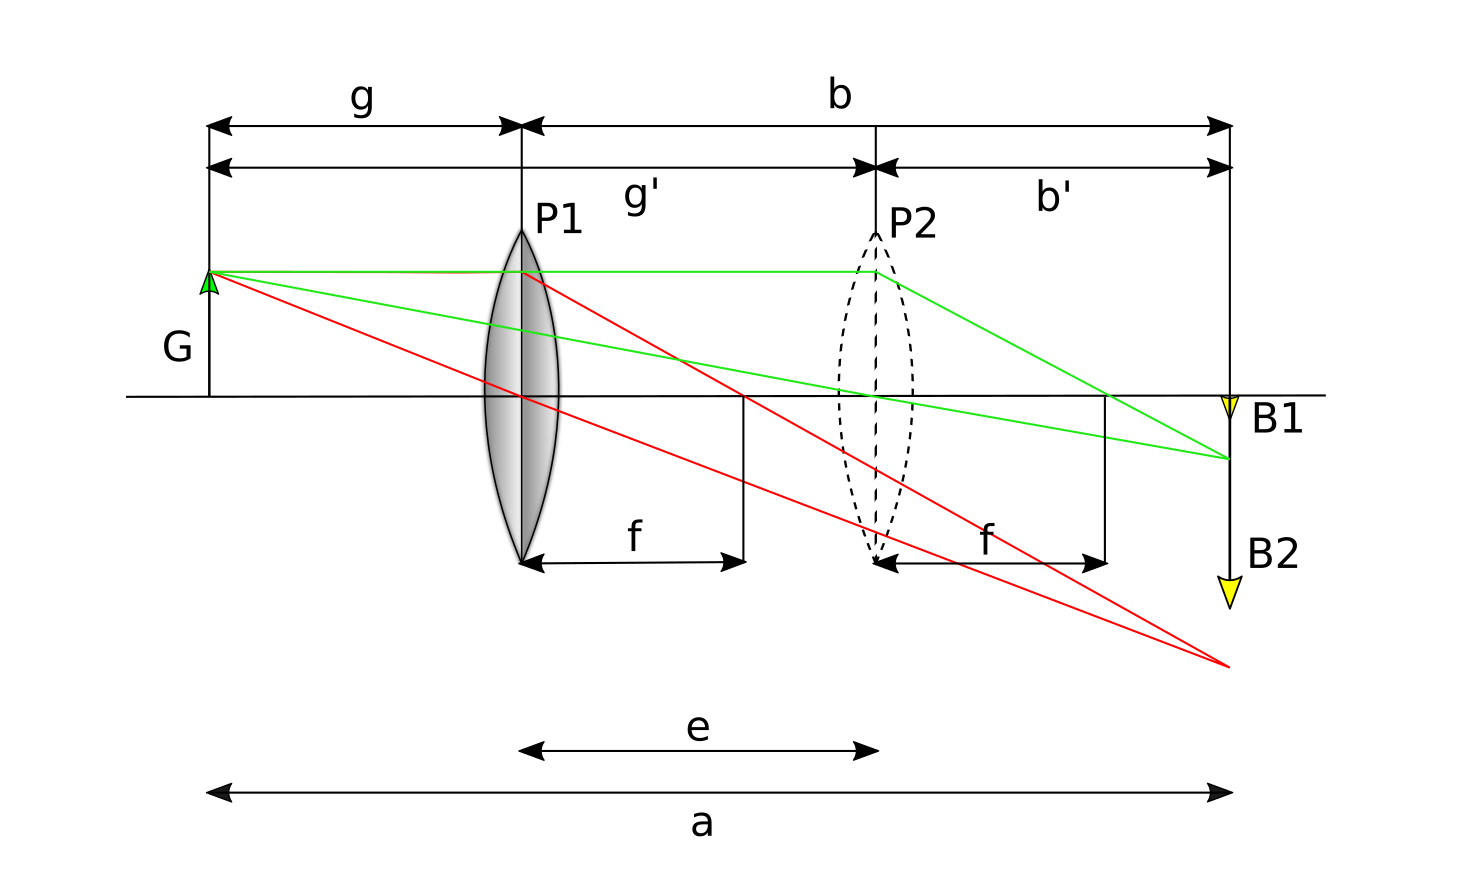
\includegraphics{Geometrische_Optik/Protokoll/fig/Besselverfahren.png}
    \caption{Besselverfahren}
    \label{fig:Besselverfahren}
\end{figure}

Zur genaueren Bestimmung der Brennweite einer dünnen Linse ist das Besselsche Verfahren gut geeignet. Dazu werden Bild (in unserem Fall ein Dia), Schirm und Linse wie in Abb. (\ref{fig:Besselverfahren}) gezeigt angeordnet. Hierbei macht man sich zu Nutze, dass es bei einem festen Abstand zwischen Bild und Schirm zwei mögliche Linsenstellungen gibt, bei denen ein scharfes Bild auf den Schirm geworfen wird. Dies soll im folgenden durch eine Herleitung gezeigt werden.
Mit einsetzen der Relationen in Gleichung \ref{Relation} in die Linsengleichung \ref{Linsengleichung}, die leicht geometrisch einzusehen ist, erhält man Gleichung \ref{Gleichung}. Diese wird für $g$ gelöst, wobei die Differenz von $g$ und $g'$ als e definiert wird (\ref{Defe}). Nach einer weiteren trivialen Umformung erhält man die Gleichung \ref{Gleichungf} für $f$.\\

\begin{equation} \label{Linsengleichung}
    \frac{1}{f} = \frac{1}{b} + \frac{1}{g}
\end{equation}

\begin{align} \label{Relation}
    b &= a - g   \\
    \nonumber b &= \frac{a-e}{2} 
\end{align}

\begin{equation} \label{Gleichung}
    \frac{1}{f} = \frac{a}{ag-g^2}
\end{equation}

\begin{equation} \label{Defe}
    e = \Delta g = \sqrt{a^2-4af}
\end{equation}

\begin{equation} \label{Gleichungf}
    f = \frac{a^2-e^2}{4a}
\end{equation}

Aus Gleichung \ref{Defe} ist sofort ersichtlich, dass für eine reelles Ergebnis $a^2 \geq 4af$ gelten muss. Außerdem ist aus selbiger auch ersichtlich, dass es nicht vorteilhaft ist $\frac{e}{f}$ zu groß zu wählen, da im Grenzfall $e = a$ gilt und somit die Linse im Bild bzw. Schirm stehen müsste. \\
Abgesehen von der eigentlichen Brennweitenbestimmung werden in diesem Versuchsteil auch zwei Linsenfehler genauer betrachtet:\\
Die chromatische und die sphärische Abberation. Dazu werden bei der Brennweitenmessung für die chromatische Rot- und Blaufilter und für die sphärische Abberation Ring- und Lochblende verwendet.\\
Bei der chromatischen Abberation handelt es sich um die Eigenschaft von Linsen, aufgrund von Dispersion, also der Abhängigkeit der Brechzahl von der Wellenlänge, beispielsweise blaues Licht stärker zu brechen als rotes. Man verwendet hier Farbfilter um die Brennweite von blauem und rotem Licht unabhängig zu messen und somit die chromatische Abberation zu bestimmen (\ref{fig:Chromatische Abberation}).\\
Die sphärische Abberation ist ein Linsenfehler bei dem, im Normalfall, achsennahes Licht weniger stark gebrochen wird, als achsenfernes Licht. Die Brennweite für achsenahes Licht fällt also größer aus, als die Brennweite für achsenfernes Licht. Um diesen Linsenfehler qualitativ zu beschreiben werden in zwei Messungen jeweils eine Loch- bzw. Ringblende vor der Linse fixiert und damit für achsennahes und achsenfernes Licht separat die Brennweiten gemessen (\ref{fig:Sphärische Abberation}).\\
Es wird jeweils einmal für den Blaufilter, Rotfilter, Ringblende und Lochblende ein Set mit je 4 unabhängigen Messungen für die beiden möglichen Kofirugationen (kleineres und größeres scharfes Bild) erstellt, wobei die ersten zwei Messungen von Person 1 und die anderen zwei von Person 2 durchgeführt wurden um personenabhängige Fehler einzugrenzen. Von jedem der insgesamt 8 Sets wird der Mittelwert ermittelt und daraus die entsprechende Brennweite errechnet.

\begin{figure}[h!]
    \centering
    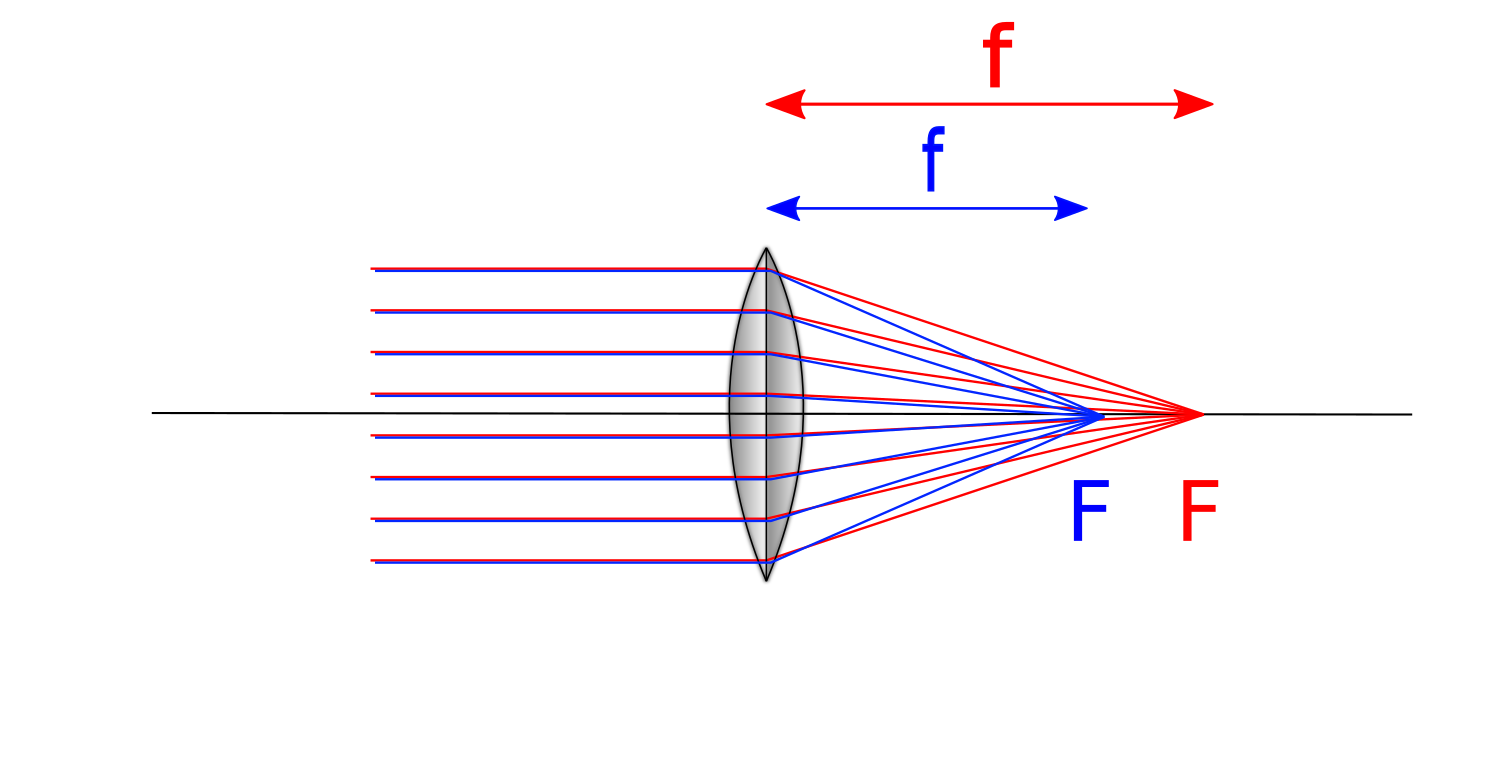
\includegraphics[scale=0.8]{Geometrische_Optik/Protokoll/fig/Chromatische Abberation.png}
    \caption{Chromatische Abberation}
    \label{fig:Chromatische Abberation}
\end{figure}

\begin{figure}[h!]
    \centering
    \includegraphics[scale=0.8]{Geometrische_Optik/Protokoll/fig/Sphärische Abberation.png}
    \caption{Sphärische Abberation}
    \label{fig:Sphärische Abberation}
\end{figure}

\clearpage

\subsection{Fehlerrechnung zur Brennweitenbestimmung einer Linse mit dem Besselverfahren}
Der Fehler wird aus der Ungenauigkeit des Maßstabs, die als $0.5mm$ (halbe Skala) abgeschätzt wird und aus dem ungenauen Winkel der Halterungen, abgeschätzt, wobei für letzteres ein Winkel von einem halben Grad als sinnvolle Ungenauigkeit erachtet wird und die Linsen ungefähr auf einer Höhe von $150mm$ angebracht sind. Somit ergibt sich insgesamt eine Ungenauigkeit von $0.5mm + \sin{0.5} = 1.5mm$
Für den Fehler auf die Mittelwerte gilt allgemein: $\sigma = \sigma_x / \sqrt{N}$ wobei $\sigma$ der resultierende Fehler ist, $\sigma_x$ der Fehler auf die Einzelmessung und $N$ die Anzahl der Messungen, wir erhalten folglich einen Fehler von $0.75mm$.
Mit der gaußschen Fehlerfortpflanzung erhalten wir für den Abstand zwischen den möglichen Linsenstellungen $e$ und für die Brennweite $f$:

\begin{equation}
    \sigma_f = \sqrt{\sum_{j=1}^m(\frac{\partial f}{\partial x_j})^2 \cdot \sigma_{x_j}^2} 
    =\sqrt{(\frac{\partial f}{\partial a})^2 \cdot \sigma_{a}^2 + (\frac{\partial f}{\partial a})^2 \cdot \sigma_{a}^2} 
    =\sqrt{\frac{1}{4}(1+(\frac{e}{a})^2)^2 \cdot \sigma_a + (\frac{-e}{2a})^2 \cdot \sigma_e}
\end{equation}

\begin{equation}
    \sigma_e
    =\sqrt{(\frac{\partial e}{\partial g_1})^2 \cdot \sigma_{g_1}^2 + (\frac{\partial e}{\partial g_2})^2 \cdot \sigma_{g_2}^2} 
    =\sqrt{(\sigma_{g_1})^2 + (\sigma_{g_2})^2}
\end{equation}

Damit ergibt sich:\\

\begin{table}[h!]
    \centering
\begin{tabular}{|c|c|c|c|c|}
	\hline
	& Blaufilter & Rotfilter & Lochblende & Ringblende \\
	\hline
	Mittelwert von e (cm) & 18.42 & 17.54 & 17.52 & 17.65 \\
	\hline
	Fehler auf e (cm) & 0.106 & 0.106 & 0.106 & 0.106 \\
	\hline
	Mittelwert von f (cm) & 13.58 & 13.71 & 13.72 & 13.70 \\
	\hline
	Fehler auf f (cm) & 0.043 & 0.043 & 0.043 & 0.043 \\
	\hline
\end{tabular}
    \caption{Mittelwerte und Fehler für e und f}
    \label{tab:Mittelwerte}
\end{table}

An den Werten der Tabelle (\ref{tab:Mittelwerte}) ist klar ersichtlich, dass es eine große Abweichung zum auf der Linse angegebenen Wert gibt, der auch nicht mehr innerhalb des Fehlers liegt. Dies kann an verschiedenen Faktoren liegen: \\

\begin{itemize}
\item die Beschriftung der Linse ist nicht korrekt
\item es wurde bei einer anderen Wellenlänge gemesse
\item es wurde deutlich näher an der Achse gemessen
\item es handelt sich um personenabhängige Fehler
\end{itemize}

Der letzte Punkt kann nahezu ausgeschlossen werden, da alle Werte nah beieinander liegen.
Auch eine große Streuung ist nicht feststellbar.\\
Eine andere Erklärung wäre, dass sich das Bild nicht zu 100\% scharf stellen lässt, da bei dieser Linse entweder der innere Bereich des Bilds scharf gestellt werden konnte oder der äußere. Außerdem lässt sich deutlich die Abweichung von dem Ergebnis der einfachen Brennweitenbestimmung erkennen, was wahrscheinlich der genaueren Messmethode zu verdanken ist.\\
Abgesehen davon kann man an den Mittelwerten, in Verbindung mit den Fehlern für die Brennweiten der einzelnen Konfigurationen, relativ deutlich die chromatische Abberation der Linse erkennen. Dahingegen lässt sich die spärische Abberation nur kaum bis gar nicht erkennen, vor allem mit dem errechneten Fehler. Daher lässt sich auf eine geringe spärische Abberation schließen.


\section{Brennweitenbestimmung eines Zweilinsensystems mit dem Abbéschen Verfahren}

\begin{figure}[h!]
    \centering
    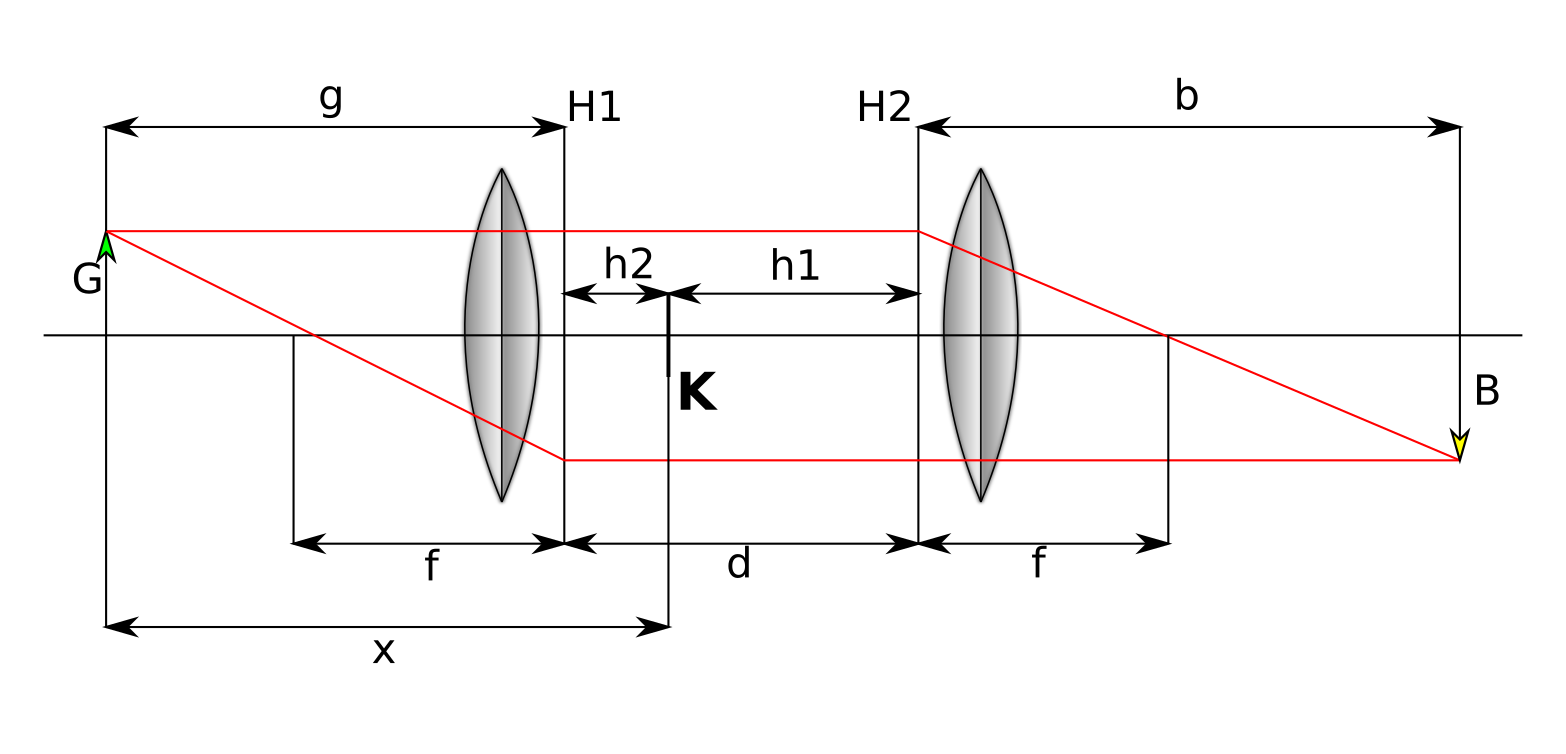
\includegraphics[scale=0.8]{Geometrische_Optik/Protokoll/fig/Abbeverfahren.png}
    \caption{Abbeverfahren}
    \label{fig:Abbeverfahren}
\end{figure}

\subsection{Fehlerrechnung zur Brennweitenbestimmung eines Zweilinsensystems mit dem Abbéschen Verfahren}